\chapter{実験結果[未完]\label{experimentalresults}}
\% 3Dプリンター作った治具での実験結果はまだ取れていないので, 出来次第随時結果をまとめていきます. 
\newpage
\section{概要}
本章では, 第\ref{devicesection}章の手順に従って行なった実験によって得られた実験結果を示す. また, 実験結果に関する考察も行う. 
\section{実験結果}
\begin{figure}[H]
  \begin{center}
    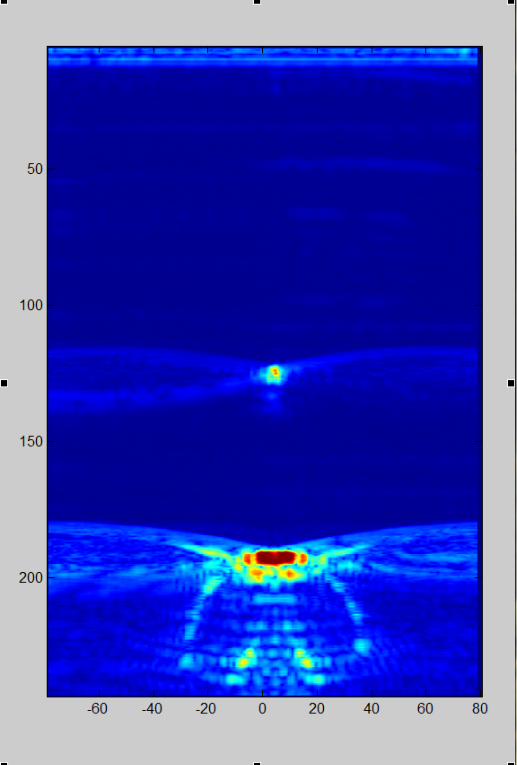
\includegraphics[width=70mm]{fig/1213_seishi_echo.pdf}
  \end{center}
  \caption{リアルタイムのエコー画像のキャプチャ}
  \figlab{1210seishi_echo}
\end{figure}
\begin{figure}[H]
  \begin{center}
    \includegraphics[width=110mm]{fig/1211_seishi_jet_2.pdf}
  \end{center}
  \caption{ジェット}
  \figlab{1210seishi_jet}
\end{figure}
\begin{figure}[H]
  \begin{center}
    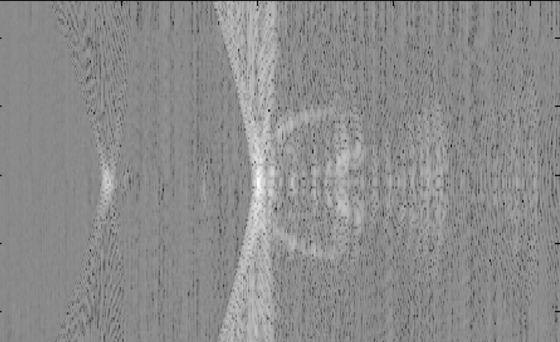
\includegraphics[width=70mm]{fig/1211seishi.pdf}
  \end{center}
  \caption{RF信号による再構成画像}
  \figlab{1210seishi_echo}
\end{figure}